\chapter{Analyse}

\section{Objectifs principaux}

Le premier point sera de récupérer un flux vidéo capturé en direct (webcam, appareil photo ou caméra) et de l'afficher tel quel.
Un autre objectif sera de permettre à l'utilisateur de prendre des instantanés du rendu vidéo et de l'enregistrer au format PNG.
De plus, nous souhaitons offrir à l'utilisateur la possibilité de modifier le rendu vidéo en temps réel et ce par le biais de différents panels de réglages identifiés par les thèmes suivants : Colorimétrie, Filtre, Effets spéciaux et Animation.
Les deux premières catégories seront composées de slider, de spinbox et de boutons, comme illustré dans la Figure \ref{maquette_parametres}. Tous les réglages pourront être réalisés et appliqués simultanément. 
Les deux catégories suivantes, quant à elles, seront représentées comme dans la Figure \ref{maquette_animation}. L'utilisateur ne pourra utiliser qu'un seul effet spécial à la fois mais pourra cumuler autant d'animations qu'il le souhaite.

\begin{figure}[h]
  \centering
  \includegraphics[width=\textwidth]{./images/P2_Maquette_Parametres.jpg}
  \caption{Maquette des paramètres}
  \label{maquette_parametres}
\end{figure}

\begin{figure}[h]
  \centering
  \includegraphics[width=\textwidth]{./images/P2_Maquette_Animations.jpg}
  \caption{Maquette des animations}
  \label{maquette_animation}
\end{figure}

\subsection{Colorimétrie}

La colorimétrie permettra de retravailler le rendu visuel de l'image à proprement parlée. Celle-ci comprendra :

\textbf{ Principaux : }

\begin{itemize}
  \item Balance des couleurs;
  \item Exposition;
  \item Gestion des tons (sombre / clair);
  \item Luminosité ainsi que le contraste
  \item saturation
  \item Température des couleurs
  \item Teinte chromatique
  \item Teinte de saturation
\end{itemize}

\textbf{ Optionnels : }

\begin{itemize}
  \item Travail par courbe
  \item Travail par niveau
\end{itemize}

\subsection{Filtres}

Les filtres permettront d'appliquer une liste d'effets en complément des réglages colorimétriques.

\textbf{ Principaux : }

\begin{itemize}
  \item Bruit
  \item Désentrelacer
  \item Fish Eye effect
  \item Flou gaussien
  \item Flou lenticulaire
  \item Flou cinétique
  \item Kaléidoscope
  \item Lissage
  \item Mosaïque
  \item Relief
  \item Zoom
\end{itemize}

\textbf{ Optionnels : }

\begin{itemize}
  \item Artistiques (Supernova, dessin au crayon, bande dessinée, ruissèlement, stroboscope, rainbow)
  \item Rendu fractal
\end{itemize}

\subsection{Effets spéciaux}

Les effets spéciaux viendront donner un corps à la modification de la vidéo en transformant significativement cette dernière.

\textbf{ Principaux : }

\begin{itemize}
  \item Endless
  \item Mirroring
  \item Slit scan
\end{itemize}

\textbf{ Optionnels : }

\begin{itemize}
  \item Face swap
\end{itemize}

\subsection{Animations}

Les animations seront des additions d'éléments externes à la vidéo. Il y en aura principalement deux types. Le premier sera de faire bouger une ou plusieurs icônes de 40x40 pixels en suivant des patterns définis ou aléatoires.

\textbf{ Principaux : }

\begin{itemize}
  \item Arabesque
  \item Bouncing (Logo DVD)
  \item Rectiligne
  \item Spiral
\end{itemize}

\textbf{ Optionnels : }

\begin{itemize}
  \item Faire défiler du texte
\end{itemize}

Le deuxième sera l'utilisation de gifs laissés au choix de l'utilisateur.

\textbf{ Principaux : }

\begin{itemize}
  \item Entrée de champs (point d'entrée défini par l'utilisateur)
  \item Fondu
  \item Traversant
\end{itemize} 

\section{Objectifs secondaires}

Au travers de ce projet, nous souhaitons devenir plus intime avec le concept d'expérience utilisateur.
Dans un tout autre registre, nous voulons nous confronter à la problématique des ralentis, l'idée est de réussir à avoir un ralenti sans pour autant augmenter le délai capture/diffusion.
Finalement, nous souhaitons explorer notre créativité au travers d'ajout de filtres et d'effets spéciaux.

\section{Objetifs tertiaires}

Si le temps nous le permets nous aimerions également pouvoir nous pencher sur le travail du son, ajout d'une soundboard mais aussi applications de divers filtres sonores.

\newpage

\begin{landscape}

\section{Planification initiale}

\begin{figure}[h]
  \centering
  \includegraphics[width=\textwidth]{./images/gantt.PNG}
  \caption{Planification GANTT}
  \label{gantt}
\end{figure}

\end{landscape}

\newpage

\begin{landscape}

\section{Diagramme des cas d'utilisation}

\begin{figure}[h]
  \centering
  \includegraphics[width=\height]{./images/useCase.png}
  \caption{Diagramme des cas d'utilisation}
  \label{useCase}
\end{figure}

\end{landscape}

\section{Technologies utilisées}

Il faut détailler le context du projet, les besoins, les spécifications, etc.

Quelle est la motivation derrière ce projet ? Qu'est-ce que ce projet apportera au final ?

On peut rajouter un diagramme WBS pour donner un aperçu haut-niveau :
\begin{figure}[h]
    \centering
    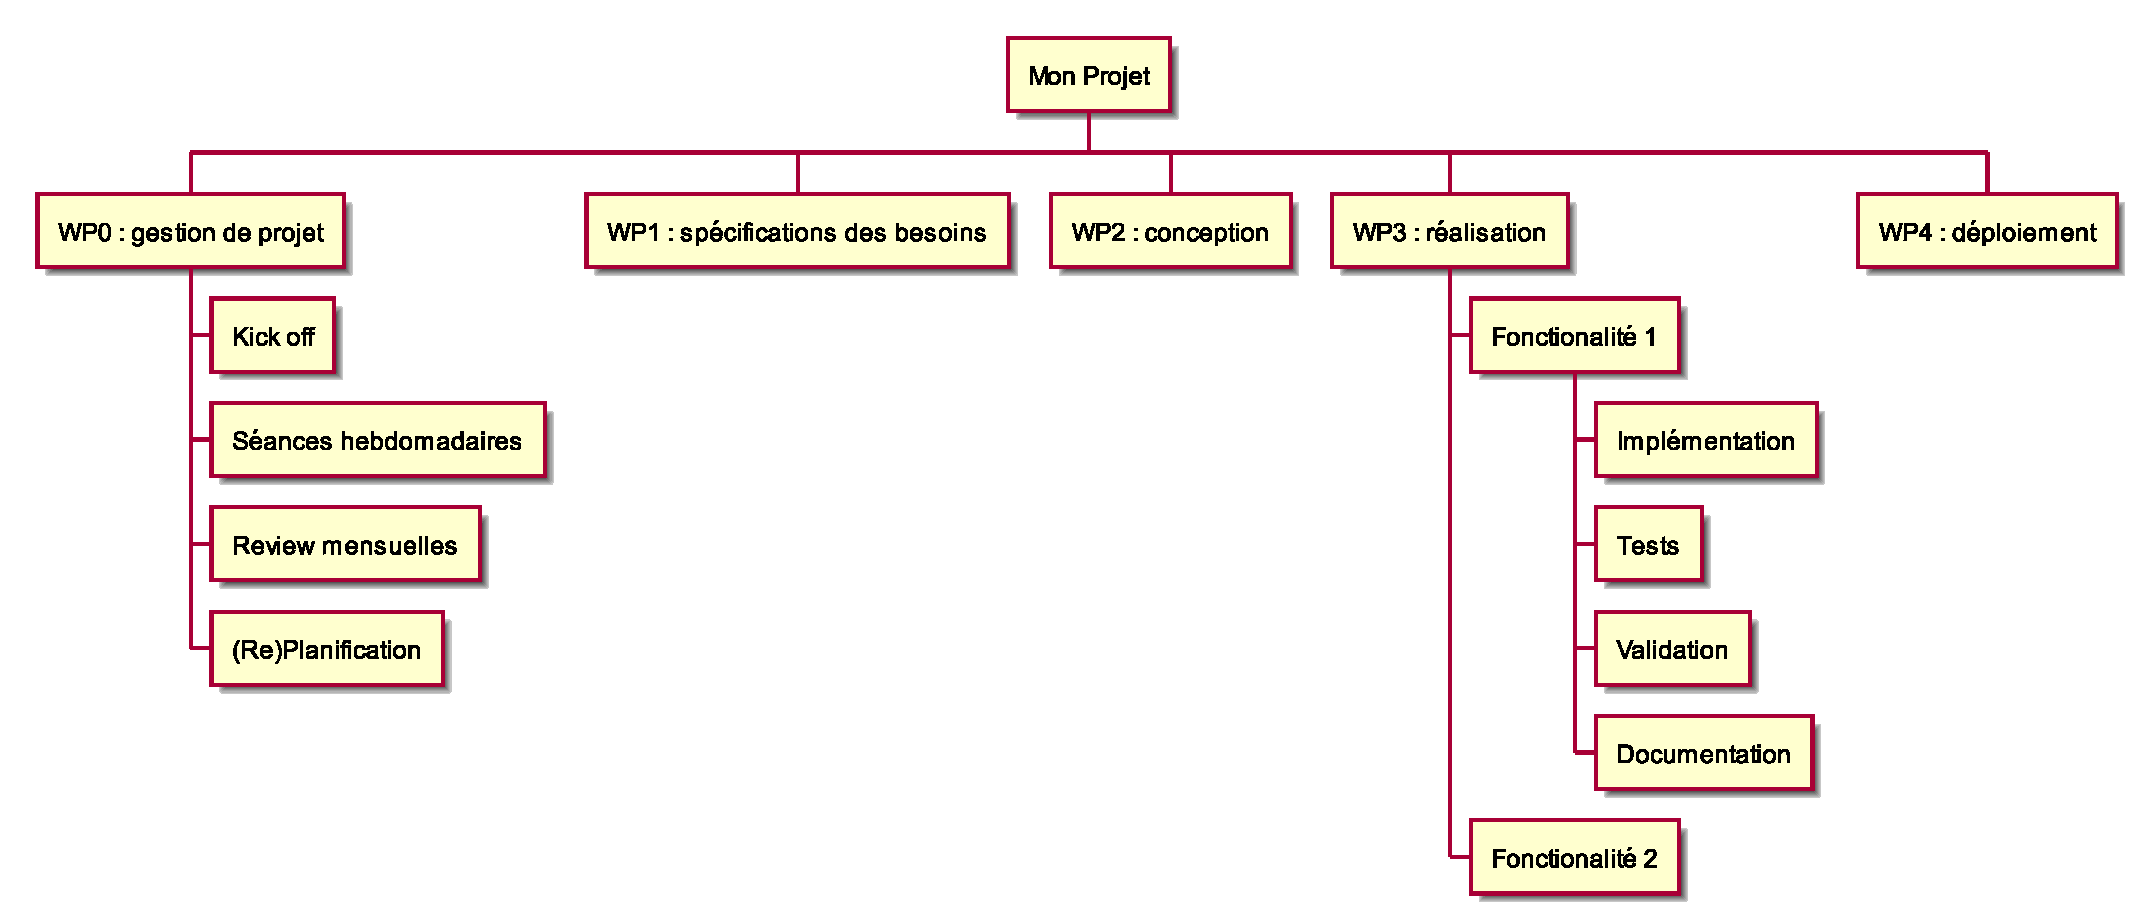
\includegraphics[width=\textwidth]{./images/WBS_Exemple.eps}
    \caption{Diagramme WBS qui va bien.}
\end{figure}

\section{Faisabilité}
Quels sont les contraintes de ce projet ? En quoi elles sont surmontables ? Un preuve de concept existe-t'elle déjà ?

\section{Risques}
Faire une analyse de risques et donner les solutions envisagées le cas échéant.
Pour chaque risque, il faut détailler les informations suivantes :
\begin{itemize}
  \item Son numéro;
  \item Son nom;
  \item Sa description;
  \item Sa probabilité : très improbable, improbable, probable, très probable;
  \item Son impact :  faible, modéré, grave, très grave;
  \item Niveau de criticité (Probabilité * Impact)
  \item Les mesures de prévention
  \item Les mesure de correction
\end{itemize}

Ensuite, on peut résumer ces informations dans un tableau comme ce qui suit :

\begin{tabular}{ | l | l | l | l | }
  N° & Nom & Probabilité & Impact \\
  \rowcolor{red!60}
  01 & Risque critique & probable & grave \\
  \rowcolor{red!20}
  02 & Risque acceptable & probable & faible \\
  03 & Risque insignifiant & peu probable & faible
\end{tabular}